
\subsection{Shape Initialization}\label{sec:initialization}

\cxj{re-write this section. Describe clearly about the parameters, the objective, and methods. }
In this section we explain the reason why using a specific angle to each fold edge, and constructing our initialized model. The basic idea is to interpret the folded state of a box as a series of rotation angles along each edge, where the problem of predicting the folded state is turned into a problem of predicting these angles.

Observe from existing data, two common rules are summarized as our basic idea of initialization.



\noindent
\textbf{Perpendicularity of adjacent faces.} Generally speaking, the adjacent planes should not be paralleled in the 3D carton model. 
To generate a box-like shape, we encourage each pair of adjacent faces to be perpendicular. 
%
This is defined as a cost term:
\begin{equation}
\alpha_{pe} = \sum_{i = 1}[\sin^{-1}(\mathbf{n}_1 \cdot \mathbf{n}_2)]^{2},
\label{equ:perp}
\end{equation}
where $\hat{n}_1$ and $\hat{n}_2$ denotes all possible combinations of normals of adjacent planes, and $n$ is the number of such combinations.

\noindent
\textbf{Plane parallelism} It was observed that two planes with same shape are probably paralleled, so we encourage more planes with same shape to be paralleled. The term is
\begin{equation}
\alpha_{pa} = \sum_{i = 1}^{n} [\cos^{-1}(\mathbf{n}_1 \cdot \mathbf{n}_2)]^{2},
\label{equ:para}
\end{equation}
where $\hat{n}_1$ and $\hat{n}_2$ denotes all possible combinations of normals of disadjacent planes that have same shape,  and $n$ is the number of such combinations.

By implementing the CMA-ES(Covariance Matrix Adaptation Evolution Strategy)~\cite{CMAES} adding the above two constrains, the initialization result is shown in Figure~\ref{fig:initial}. Note that as the input variables are fold angles of edges, $\mathbf{n}_1 \cdot \mathbf{n}_2$ is represented by $cos\alpha$ where $\alpha$ is the angle between these two normal vectors. 

We can see from the five examples shown in Figure~\ref{fig:initial}, the up three examples can have ideal results and the bottom two results are even not closed at last, which actually caused by the two constrains above lead to a result that each angle of each edge is always $\pi/2$. As a consequence, some irregular boxes will present a boxy shape which will be refined later by user interaction.

As for our initialization, $\pi/2$ is finally set to each angle and this causes more than half of boxes folded correctly in our database.


\cxj{do not use angle. do you use parallelism?}
%\begin{figure}
%	\centering
%	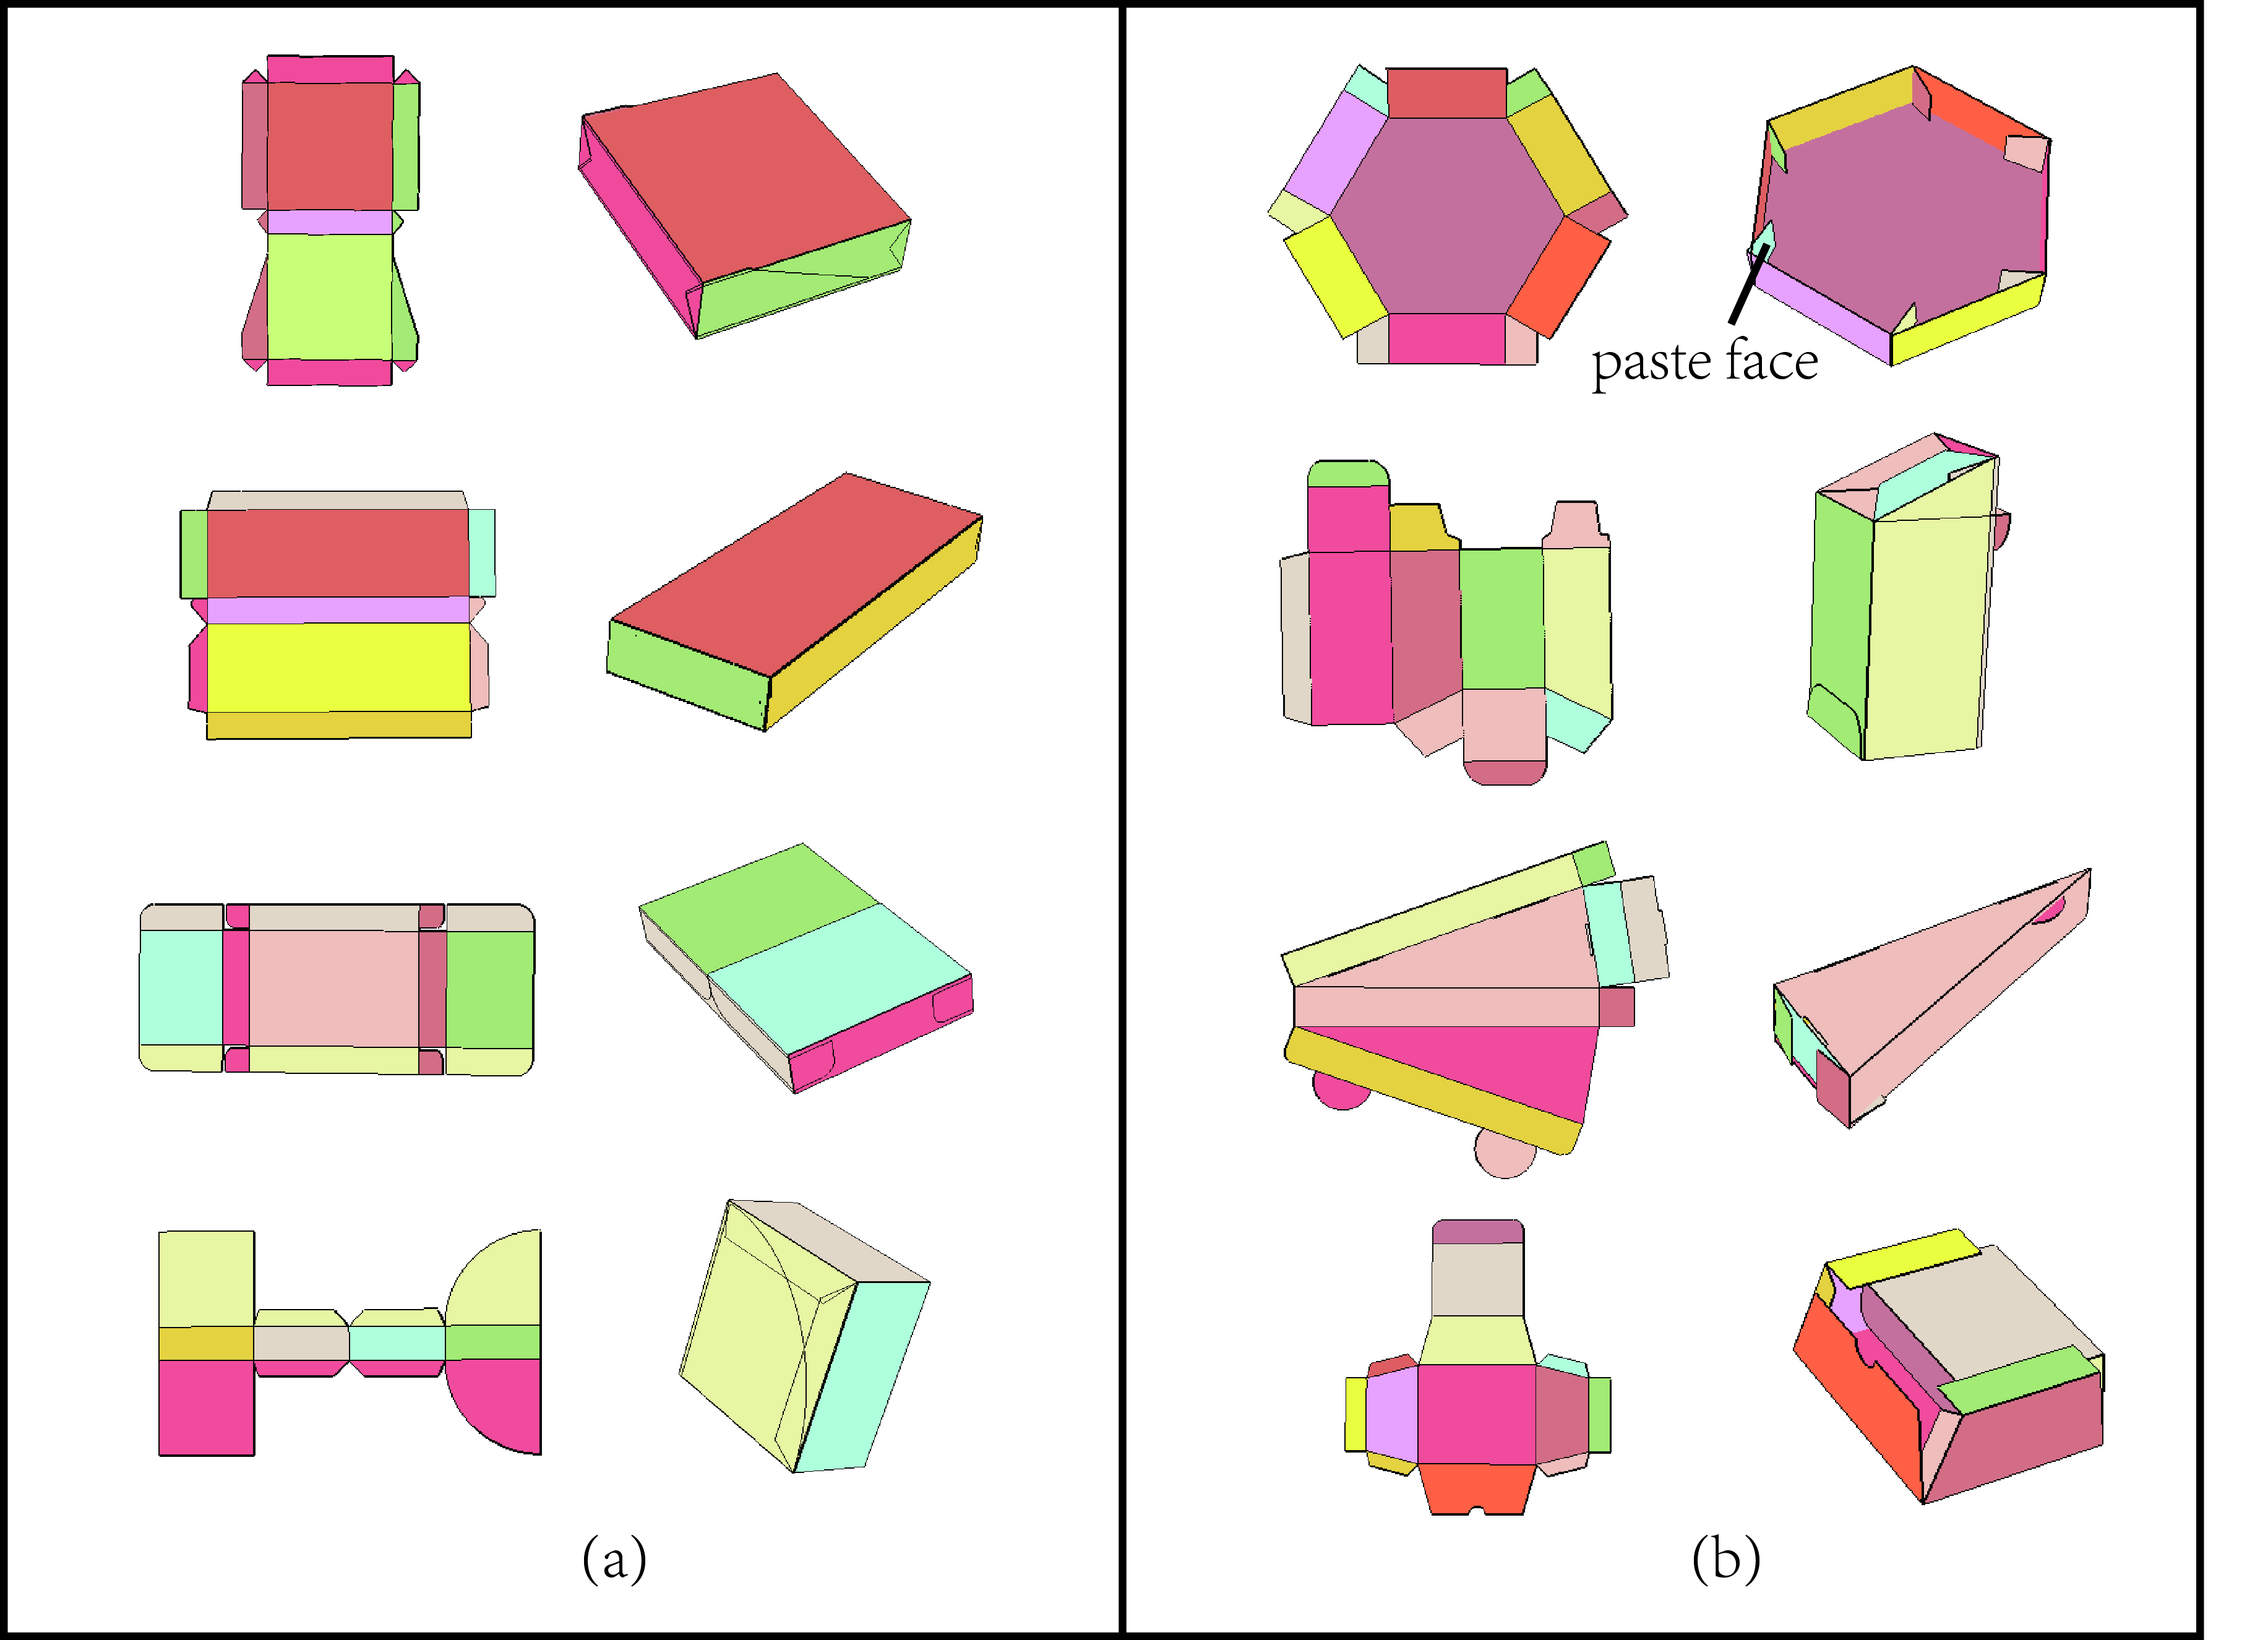
\includegraphics[width=0.9\textwidth]{images/initial.jpg}
%	\caption{Initialized results of five examples. Each row is an example, and the first column is the 2D design layout, the second column is the polymesh created from layout, the third column is the initialized results optimized with the two constrains.}
%	\label{fig:initial}
%\end{figure}

\begin{figure}
	\centering
	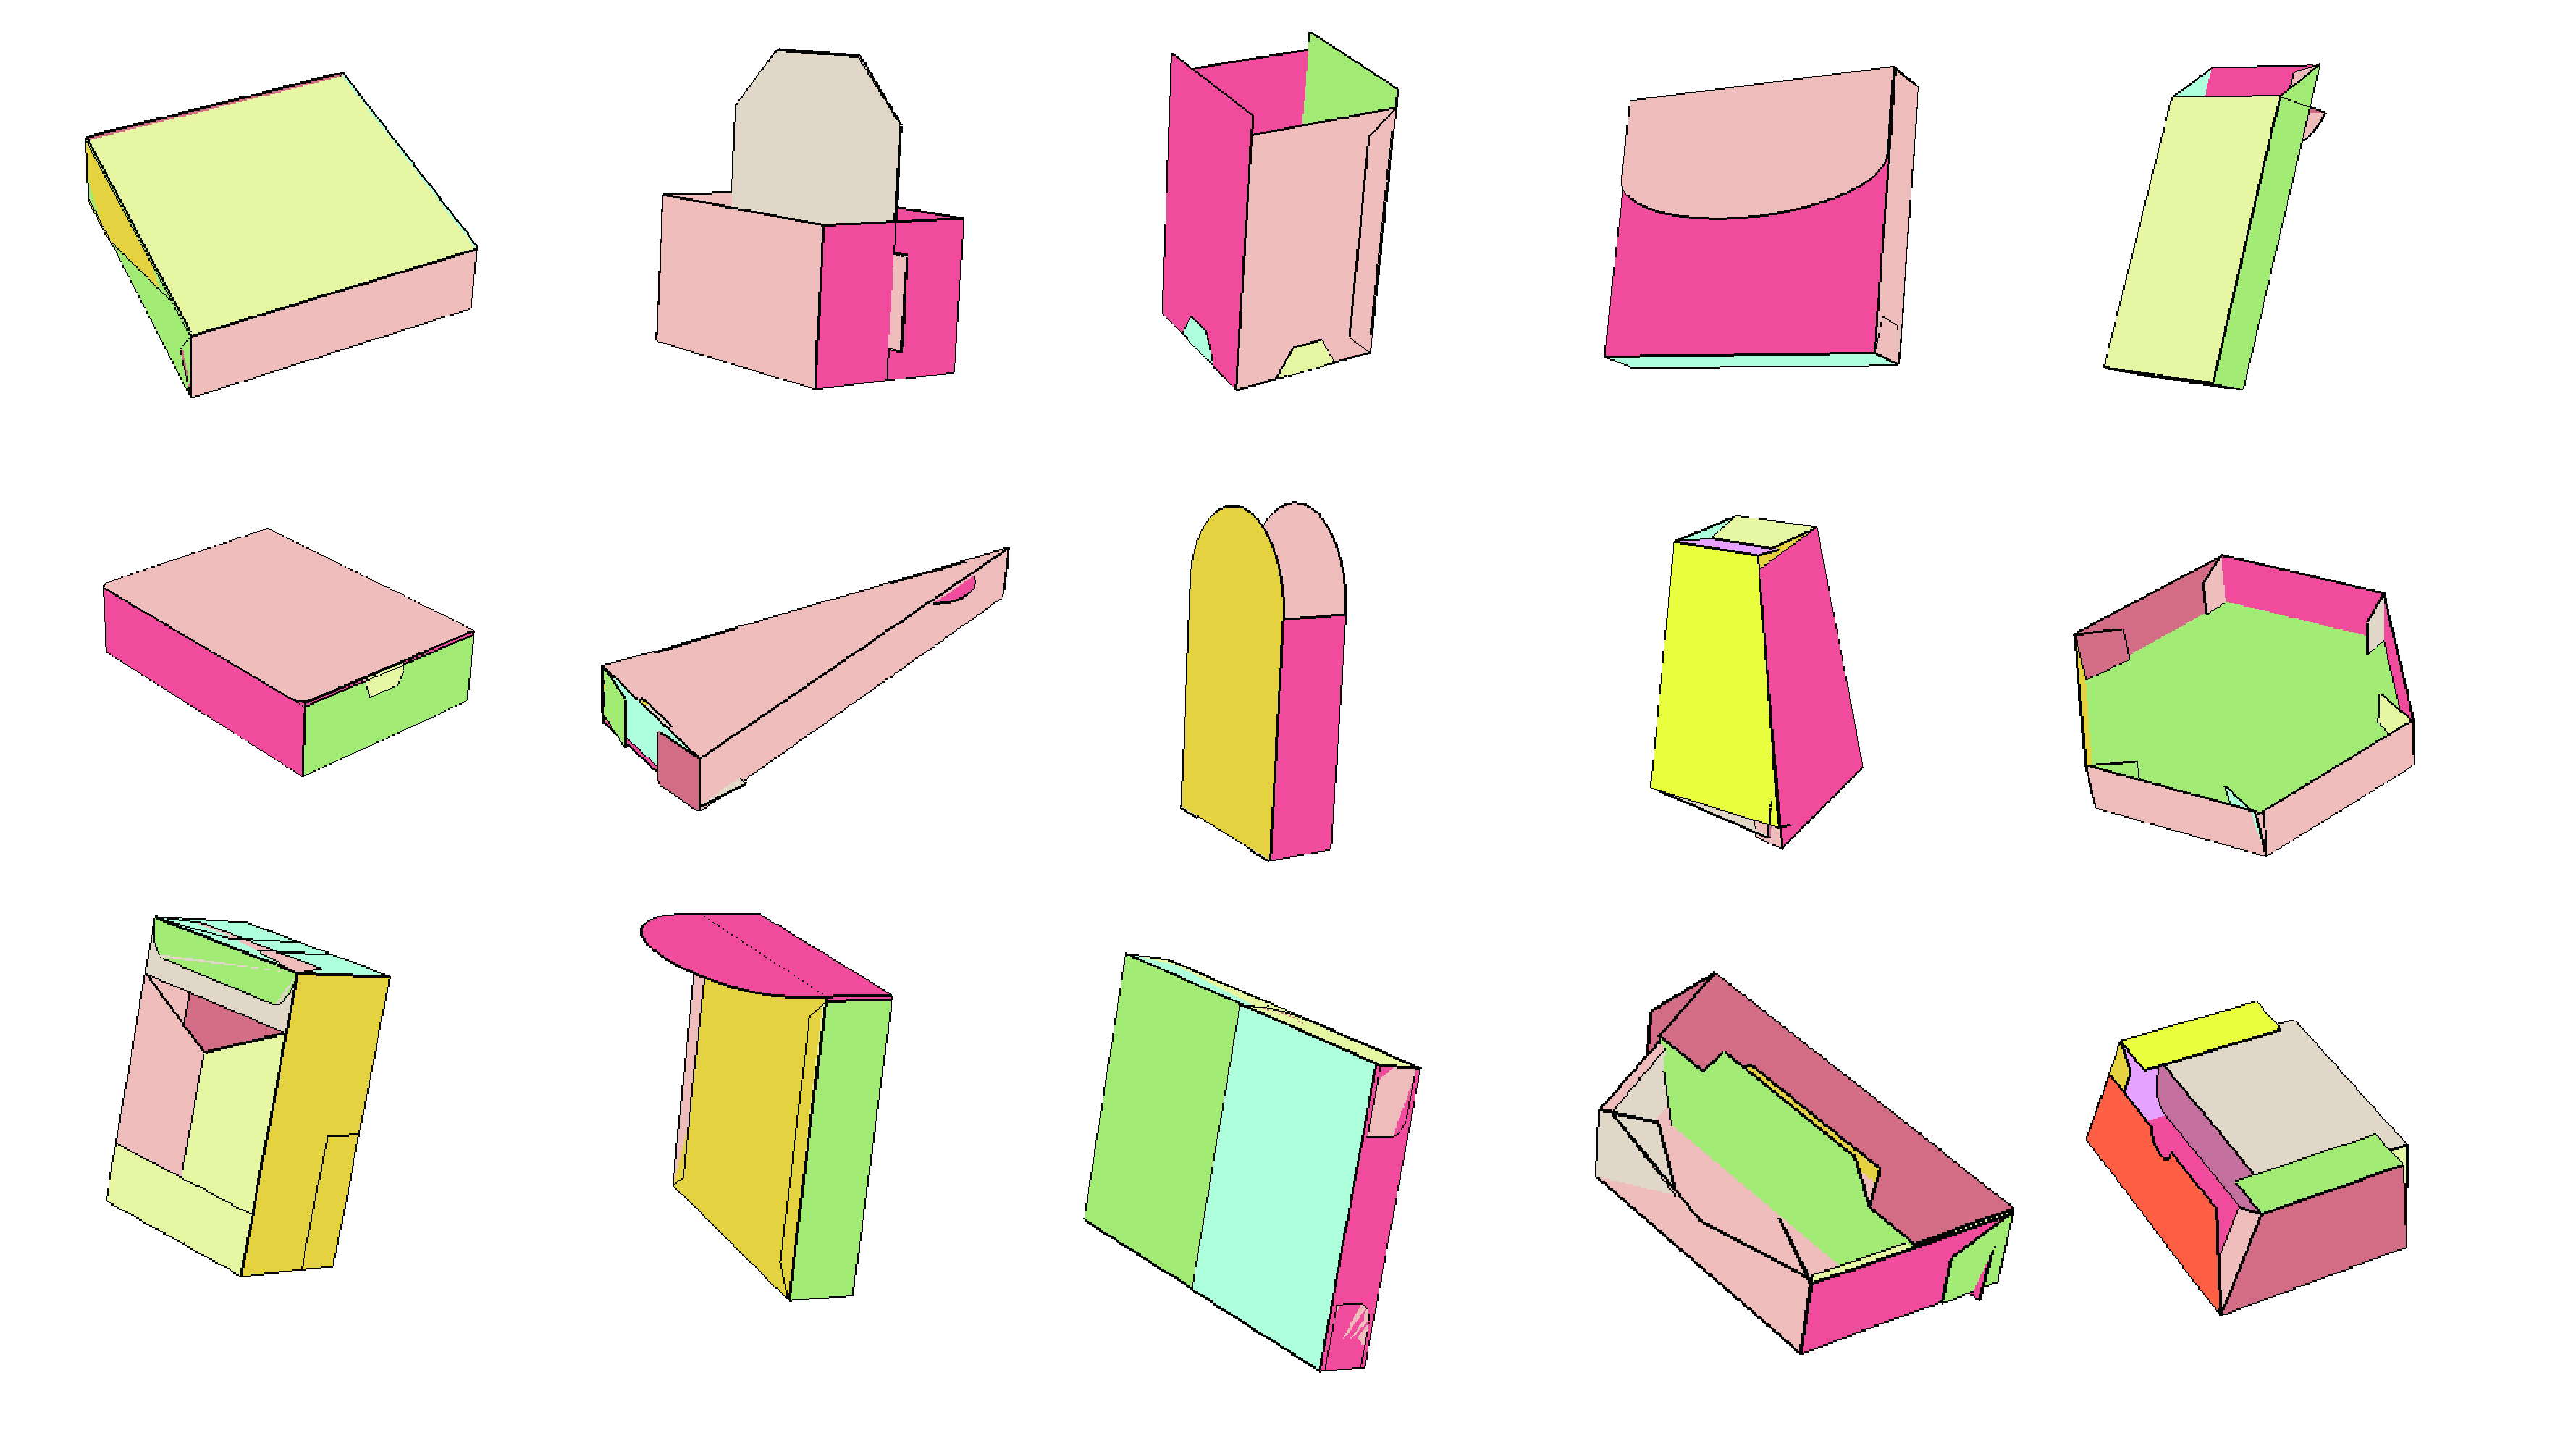
\includegraphics[width=0.9\textwidth]{images/initial2.jpg}
	\caption{15 different initialization results. Eight of them need not further refine. \cxj{show the input. point out which 8.}}
	\label{fig:initial}
\end{figure}

%%%%%%%%%%%%%%%%%%%%%%%%%%%%%%%%%%%%%%%%%%%%%%%%%%%%%%%%%%%%%%%%%%%%%
